% -*- Mode: LaTeX; Mode: Flyspell -*-

\section{Introduction}

\paolo{
The provenance of data is a form of structured metadata that records the processes involved in data production. In addition to references to data generation or transformation processes, a \textit{provenance trace} may include input  or intermediate data products, as well as references to agents, humans as well as software systems, who were responsible for those processes.
%
	In multi-party collaboration settings that involve data sharing, as well as in third party auditing of data and processes, there is a broad expectation that 
shipping the available provenance to collaborators, or more generally publishing it along with the data, may help data consumers form judgements regarding the reliability of the data itself.
}

%
\paolo{
	Offering to disclose the provenance of a data as evidential basis for establishing data quality and reliability is particularly important when data products are exchanged as part of transactions amongst parties with limited mutual trust. 
This is the case for instance of \textit{dynamic coalitions}~\citep{BFJM06}, ad hoc collaborative partnerships that are created 
to pursue a common goal, in scenarios such as multi-agency emergency/threat responses, as well as the exchange of intelligence information. 
Despite the need to share data of a possibly sensitive nature, these coalitions are characterized by a lack of established interaction protocols and by limited trust amongst the partners. 
}
\paolo{
This situation creates a tension between data providers and consumers, when it comes to negotiating the level of detail of the orovenance that providers are prepared to offer to consumers. 
On one hand, consumers will require as much provenance detail as possible.
Data providers, however, will be reticent to offer detailed provenance traces, because those may contain sensitive information regarding their own internal processes as well as any proprietary data used by those processes.
%
To appreciate how such tension may arise, consider the following scenario, where ...  
%
}
\paolo{TBD -- rewriting the example in 1.1. removed fig 1} \\




\paolo{OLD TEXT BELOW}

%Second, regarding \textit{selective disclosure}, we are motivated by the emerging notion of .
%
%
%
Our working assumption is that, in this setting, provenance can be used as a form of evidence in support of the data that is being exchanged. 
%
In these scenarios, full disclosure of provenance data may not be possible, e.g. due either to confidentiality policies, Intellectual Property restrictions associated with individual components, or data protection regulations. These restrictions introduce the need to hide certain parts of the provenance traces. 
%
In this paper we develop a model and algorithm for performing  abstraction over provenance metadata. These provide the theoretical underpinning, defined on top of PROV, for applications that require provenance exchange while obfuscating some of its content.

%The work presented in this paper is motivated 

The recent standardisation of a data model for exchanging provenance in an interoperable way, namely the PROV model from the W3C~\citep{w3c-prov-dm}, makes this assumption realistic.
%


%controlling the selective disclosure of potentially sensitive provenance content

%In this paper we address the problem of controlling the selective disclosure of provenance information, which may arise in the presence of limi
With the emergence of provenance as a valuable complement to data in such a setting, two separate but related issues arise, namely that of interpretation of complex provenance by humans,  and that of .
  
%
First, regarding \textit{complexity}, we observe that while provenance is a rich form of metadata, it is often the reflection of articulated processes involving many intermediate data products and many inter-related activities. 
%
Such complexity is at odds with the need for humans to understand the meaning of the data, common for instance in e-science. 
While provenance is an important element of scholarly communication, it needs to be understandable by non-technical users, i.e., scientists. 
%
Indeed in e-science, the idea of abstracting provenance to make it understandable is not entirely new.
%
The Zoom system~\citep{DBLP:conf/icde/BitonBDH08}, discussed in more detail below, is an example of a system for computing views over provenance, which is designed to simplify human understanding of provenance traces.
%



\subsection{Motivating scenario: provenance of intelligence information}
%
%
%\begin{figure}
%\centering
%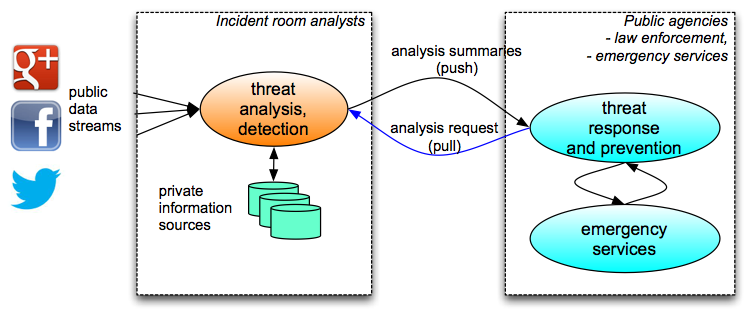
\includegraphics[scale=.35]{figures/intelligence-scenario.png} 
%\caption{Simple two-way partnership involving one sender (IR) and one receiver (PA)}
%\label{fig:scenario}
%\end{figure}

Imagine a setting where one or more public agencies engage in a business relationship with an independent intelligence provider. 
%
In Fig.~\ref{fig:scenario} these are the Public Agencies (PA) box and the Incident Room Analysts (IR) box, respectively.
%
IR has a business incentive to provide analysis of potential threats to PA that is as accurate as possible, while PA has an interest in acquiring and acting upon intelligence reports issued by IR.
%
Realistically, however, PA will want to mitigate the risk of acting upon information provided by IR, which is potentially unreliable. At the same time, IR has a business incentive to supply PA with additional evidence that facilitates PA's risk assessment.
%

%
The  key assumption that motivates our work is that the provenance of the intelligence report is relevant in contributing, at least in part, the required evidence. This may contain a wealth of details regarding how the report was produced, including the raw input data used for the analysis, the analytical tools and their configuration parameters, as well as the identity of the analysts involved, and their position within the business organization.  

%
An example of provenance containing such information is shown in Fig.~\ref{fig:graph-example}.
%
As depicted in the figure, provenance can be represented as a graph whose nodes represent either \textit{entites} (ovals in the figure), i.e., data, documents, etc., \textit{activities} (rectangles), which represent the execution of some process over a period of time, or \textit{entites} (pentagons), which represent  humans or computing systems. Directed edges represent various types of relationships, the most common being ``activity $a$ used entity $e$'', ``entity $e$ was generated by activity $a$'', ``activity $a$ was associated with agent $ag$'' (i.e., $ag$ was responsible for $a$), and more.
%
Provenance graphs are introduced more formally in Sec.~\ref{sec:prov-core}.

\begin{figure*}
\begin{center}
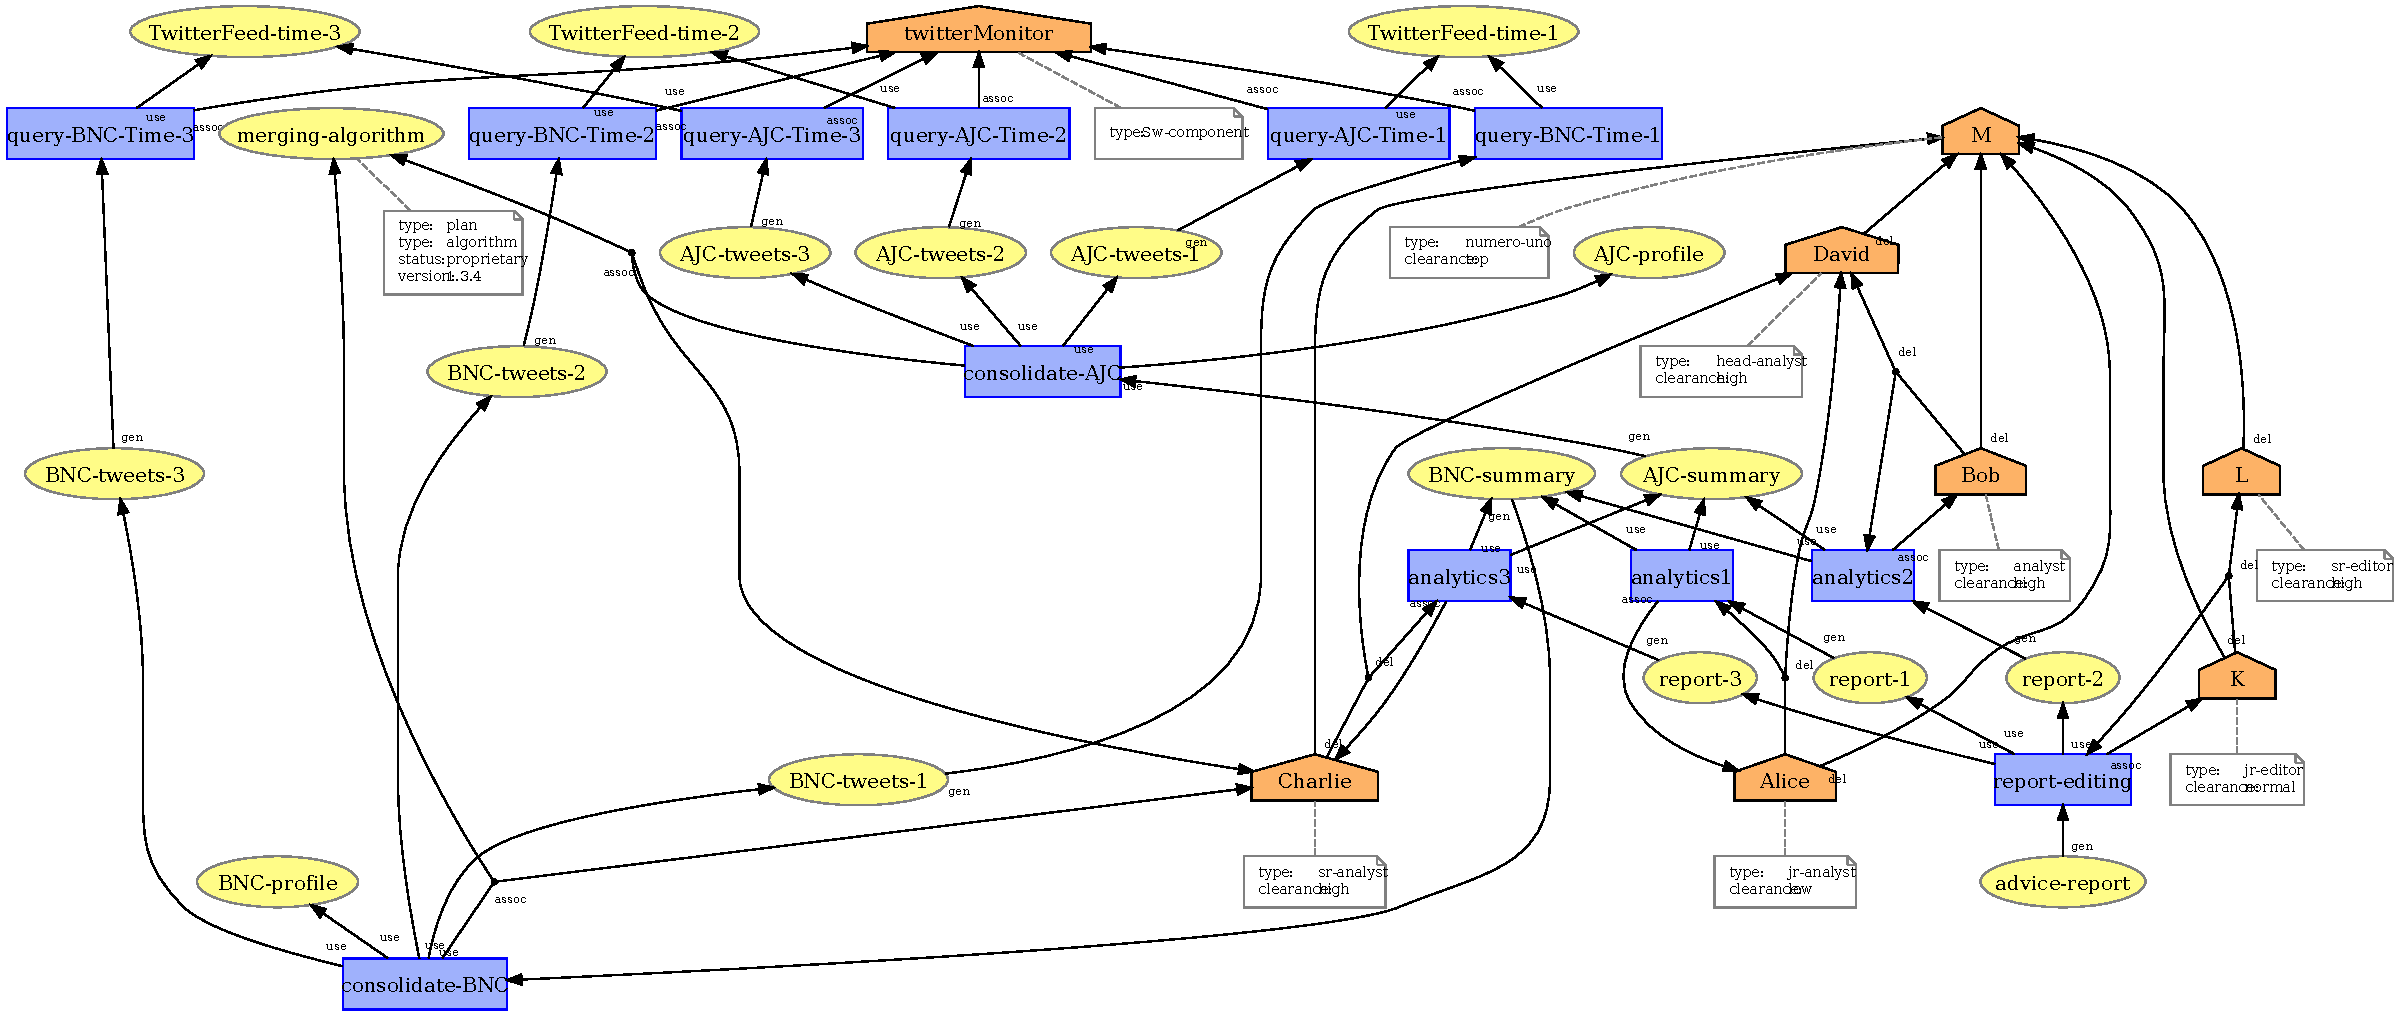
\includegraphics[width=\textwidth]{figures/IR-agents-delegation.pdf}
\caption{Example provenance graph for the reference scenario (Fig.~\ref{fig:scenario})}
\label{fig:graph-example}
\end{center}
\end{figure*}

%
While both IR and PA are interested in sending and receiving such provenance information, some of it may be sensitive and proprietary. 
%
Input datasets may include a combination of public social media streams, shown in the figure, and private databases. Likewise, analytical tools may include proprietary algorithms.
%
In a setting where mutual trust is limited, the contrast between the need to exchange provenance as a form of evidence on one side, and the need to protect confidential information that can be found in the provenance on the other, generates a tension amongst the partners.

%
We believe that such tension can be resolved by providing IR, the \textit{provenance owner}, with ways to control the disclosure of provenance to third parties. This consists of (i) a model of abstraction over provenance, whereby some of its elements are grouped together and replaced with a new, abstract element, and (ii) a policy model that the provenance owner can use to specify the  elements which are to be abstracted.
%
% These are used by the provenance owner to support a process of \emph{negotiation} with the third parties, 

The work presented here is focused exclusively on (i), while (ii)  is the subject of a separate report, focused on a user tool for the specification and enforcement of provenance abstraction policies~\citep{MBGCD14}.  
%
%
%For completeness, however, we provide a brief overview of the tool  and an example of an abstraction policy  in Sec.~\ref{sec:summary}. % Sec~\ref{sec:further} concludes.




\subsection{Options for provenance abstraction }  \label{sec:contributions}

Removal of information from a provenance graph can be achieved in a number of ways.
%
 One could simply remove the labels as well as the annotations from individual nodes and relationships, i.e., anonymize part of the graph. Doing so, however, does not hide any of the structure of the process of data production. One could further remove nodes and relationships, for instance nodes \texttt{consolidateAJC} and \texttt{consolidateBNC} in the graph of Fig.~\ref{fig:graph-example}, or  indeed entire sub-graphs. The new graph will be disconnected, however, making it difficult to reconstruct the lineage of the end data product, that is, the sequence of data derivations from the initial inputs to the outcome of the process.
 
Instead, our abstraction operator replaces a sub-graph with a new abstract node, and then ``re-wires'' the new node to the remaining original graph. This has the effect of hiding parts of the process structure as it was represented in the original provenance, while maintaining connectivity. One can still query the lineage, but some of the provenance elements returned by the query will now be an abstraction of the actual data production process.

The main challenge is to guarantee that abstraction produces PROV-compliant  graphs,   maintaining the interoperability guarantees provided from having standardized PROV and ensuring that the results can be consumed by standard PROV tools. We provide a proof of this in the Appendix.
%demonstrate this 



%compatibility with standard PROV tools can consume and 

% would be compromised.
 
%  A second option, which we take here, is to define a rewriting that generates a PROV-compliant graph.




% We view provenance abstraction as a form of graph rewriting. Conceptually, two approaches can be taken when defining the rewriting rules.
 %
% One option is to extend the PROV model  with additional elements (for instance, new types to denote abstract nodes) and a corresponding system of constraints, resulting in an extension PROV' of PROV.
 %
%  In this setting, a legal rewriting is one that transforms a valid PROV graph $\pg$ into a valid PROV' graph $\pg'$, where validity is interpreted as conformance to the PROV' schema.
  %
%  While this approach leads to the definition of a new and possibly interesting model for \textit{abstract provenance}, the interoperability guarantees provided from having standardized PROV would be compromised.
 
%  A second option, which we take here, is to define a rewriting that generates a PROV-compliant graph.
 

 
\subsection{Contributions}
Our specific contribution is the formal definition of a provenance abstraction operator that rewrites  a PROV graph $\pg$ into a new graph $\pg'$, by mapping a set $V_{gr}$ of nodes (for ``vertex in a group'') in $\pg$ to a new abstract node $v_{new}$, and then mapping each relationship involving elements of $V_{gr}$ to a new relationship involving $v_{new}$ in $\pg'$. 
We prove several formal properties of $\pg'$: firstly, schema preservation: if $\pg$ is a PROV graph, that is, it conforms to the PROV data model~\citep{w3c-prov-dm}, then $\pg'$ is also a PROV graph. Secondly, validity preservation: if $\pg$ is \textit{valid}, that is, it satisfies all PROV constraints~\citep{w3c-prov-dm}, then $\pg'$ is also valid. Finally, no spurious dependencies are introduced into $\pg'$: a  relationship involving $v_{new}$ is only created as a result of a mapping from an existing relationship involving elements of $V_{gr}$. Strictly, if $a$ and $e$ are not \textit{directly} related in $\pg$, we guarantee that they are not directly related in $\pg'$. 
Note that new indirect dependencies between two nodes in $\pg'$, manifested as new paths in the graph, may be introduced, however we show that these are always justified by the topology of the underlying graph $\pg$.

Note that, by making the abstraction operator closed with respect to the set of valid PROV graphs, abstraction can be naturally composed, i.e., one can abstract $\pg'$ into some $\pg''$.

Note also that $\pg'$ itself has also an associated provenance graph, that is, a record of the provenance abstraction process as it was applied to $\pg$. 
PROV provides a syntactic facility to maintain the association between a provenance graph and its own provenance, namely using the ``provenance of provenance'' mechanism (i.e., bundles~\citep{w3c-prov-dm}).



%
%The remainder of the paper is structured as follows. After a review of related work, in Sec.~\ref{sec:prov-core} we introduce the fragment of the PROV model that defines the scope of our work, followed by an overview of the approach and summary of contributions (Sec.~\ref{sec:overview}).
%%
%The core technical material is in Sec.~\ref{sec:grouping}, where we define abstraction over provenance in terms of a \textit{grouping} operator, present its functional specification, and show that grouping maps a graph into a new graph that conforms to the same relational schema.

